\lab{Wave Phenomena}{Wave Phenomena}
\label{lab:waveeqn}
\labdependencies{Animation,FiniteDifferenceMethod,HeatFlow}

\section*{Advection Equation}
The advection equation (or transport equation) is given by $u_t + s u_x = 0$, where $s$ is a nonzero constant.
Consider the Cauchy problem
\begin{align*}
	& u_t + su_x = 0, \quad -\infty < x < \infty,\\\
	& u(x,0) = f(x).
\end{align*}
The function $f(x)$ may be thought of as an initial wave or signal.
The general solution of this initial boundary value problem is $u(x,t) = f(x-st)$ (check this!).
The solution $u(x,t)$ is a traveling wave that takes the signal $f(x)$ and moves it along at a constant speed $s$ --- to the right if $s > 0$, and to the left if $s < 0$.

\section*{Wave Equation}
Many different wave phenomena can be described using a hyperbolic PDE called the wave equation.
These wave phenomena occur in fields such as electromagnetics, fluid dynamics, and acoustics.
This equation is given by
\begin{align}
	u_{tt} &= s^2 \nabla^2 u
\end{align}
where $\nabla^2 = \nabla \cdot \nabla$ is the Laplace operator.
The 1D equation can be derived in the context of many physical models; a common derivation describes the motion of a string vibrating in a plane.
Another nice derivation uses Hooke's law from the theory of elasticity.

After making the change of variables $(\xi,\eta) = (x-st, x + st)$ and using the chain rule, we find that the 1D wave equation $u_{tt} = s^2 u_{xx}$ is equivalent to $u_{\xi \eta} = 0$.
The general solution of this last equation is
\[u(\xi, \eta) = F(\xi) + G(\eta)\]
for some scalar functions $F$ and $G$.
In $(x,t)$ coordinates the solution is
\[u(x,t) = F(x-st) + G(x+st).\]
Thus the general solution of the wave equation is the sum of two parts: one is a signal traveling to the right with constant speed $|s|$, and the other is a signal traveling to the left with speed $|s|$.


Given two homogeneous Dirichlet boundary conditions (for the second-order spatial derivative) and two sets of initial conditions (because the second-order time derivative), the wave equation takes the form
\begin{equation}
    \begin{split}
	u_{tt} &= s^2 u_{xx}, \quad 0 < x < l, \quad t > 0,\\
	u(0,t) &= u(l,t) = 0, \\
	u(x,0) &= f(x),\\
	u_t(x,0) &= g(x).
    \label{waveeqn:eqn:wave-equation}
    \end{split}
\end{equation}

\subsection*{Numerical solution of the wave equation}
We look to approximate $u(x,t)$ on a grid of points $(x_j,t_m)_{j=0,m=0}^{J,M}$.
Denote the approximation to $u(x_j,t_m)$ by $U_{j}^{m}$.
Note that the superscipt index $m$ denotes the time index and runs from $0$ to $M$, while the subscript $j$ denotes the spatial index and runs from $0$ to $J$.
Recall that the centered approximations in space and time are
\begin{align}
	\begin{split}
		D_{tt} U_{j}^{m} &= \frac{U_{j}^{m+1} -2 U_{j}^{m} + U_{j}^{m-1}}{(\Delta t)^2} ,\\
		D_{xx} U_{j}^{m} &= \frac{U_{j+1}^{m} -2 U_{j}^{m} + U_{j-1}^{m}}{(\Delta x)^2} .
		\label{waveeqn:eqn:2nd-order-centered-2nd-derivative}
	\end{split}
\end{align}
The resulting method is given by
\begin{align*}
	&\frac{U_{j}^{m+1} -2 U_{j}^{m} + U_{j}^{m-1}}{(\Delta t)^2} = s^2 \frac{U_{j+1}^{m} -2 U_{j}^{m} + U_{j-1}^{m}}{(\Delta x)^2}, \\
	&U_{j}^{m+1} =  - U_{j}^{m-1} + 2 (1-\lambda^2) U_{j}^{m} + \lambda ^2 (U_{j+1}^{m} + U_{j-1}^{m}),
\end{align*}
where $ \lambda  =  s(\Delta t)/(\Delta x)$.
This method may be written in matrix form as
\begin{equation}
U^{m+1} = AU^{m} - U^{m-1} 
\label{waveeqn:eqn:matrix-form}
\end{equation}
where
\begin{equation*}
A =
\left[\begin{array}{cccc}2(1-\lambda^2) & \lambda^2 &  &  \\ \lambda^2 & 2(1-\lambda^2) & \lambda^2 &  \\ \ddots & \ddots & \ddots &  \\ & \lambda^2 & 2(1-\lambda^2) & \lambda^2 \\  &  & \lambda^2 & 2(1-\lambda^2)\end{array}\right]
\end{equation*}
and
\begin{equation*}
    U^m = \left[\begin{array}{c}U_{1}^{m} \\U_{2}^{m} \\\vdots \\U_{J-1}^{m}\end{array}\right].
\end{equation*}

In the matrix equation above, we have already used the boundary conditions to determine that $U_{0}^{m} = U_{J}^{m} = 0$ at each time $t_m$.
Note that, to obtain the approximation $U_{j}^{m+1}$ of $u(x_j,t_{m+1})$, the method uses the value of the approximation at \emph{the previous two time steps}.
We can find the solution for the first two time steps by using the initial conditions.
Using the initial conditions directly gives an approximation at $t = t_0 = 0$:
\[U_{j}^{0} = f(x_j), \quad 1 \leq j \leq J-1\]

To obtain an approximation at the second time step, we consider the Taylor expansion
\begin{align*}
	u(x_j,t_1) &= u(x_j, 0) + u_t(x_j,0) \Delta t + u_{tt}(x_j,0) \frac{\Delta t^2}{2} + u_{ttt}(x_j,t_1^*) \frac{\Delta t^3}{6}.
\end{align*}
Recalling that the solution $u(x,t)$ satisfies the wave equation, we substitute in expressions from our initial conditions:
\begin{align*}
	u(x_j,t_1) &= u(x_j, 0) +  g(x_j) \Delta t+ s^2 f''(x_j)\frac{\Delta t^2}{2} +  u_{ttt}(x_j,t_1^*) \frac{\Delta t^3}{6}.
\end{align*}
Ignoring the third-order term, we obtain a second-order approximation for the second time step:
\begin{equation*}
U_{j}^{1}= U_{j}^{0} + g(x_j) \Delta t+ s^2 f''(x_j) \frac{\Delta t^2}{2}, \quad 1 \leq j \leq J-1,
\end{equation*}
or if $f$ is not readily differentiable,
\begin{equation}
    U_{j}^{1}= U_{j}^{0} + g(x_j) \Delta t+ \frac{\lambda^2}{2} (U^0_{j-1} -2 U^0_j + U^0_{j+1}).
    \label{waveeqn:eqn:first-time-step}
\end{equation}
This method is conditionally stable; the CFL condition (a necessary condition for convergence of PDEs) is that $\lambda \leq 1$.

Notice that the matrix $A$ is sparse.
As such, you'll want to use sparse matrices and routines from \li{scipy.sparse}.

\begin{problem}
    \label{waveeqn:prob:solve_wave}
    Define a function \li{solve_wave} to numerically approximate solutions to equations of the form \eqref{waveeqn:eqn:wave-equation}.
    Your function should accept the following as parameters:
    \begin{itemize}
        \item a spatial domain $(x_0, x_f)$,
        \item a time domain $(t_0, t_f)$,
        \item a number of spatial intervals $J$,
        \item a number of time intervals $M$,
        \item the parameter $s$,
        \item an initial condition $f(x) = u(x, 0)$, and
        \item an initial condition $g(x) = u_t(x, 0)$.
    \end{itemize}
    Compute and return the numerical approximation $U$ as an array using equations \eqref{waveeqn:eqn:matrix-form} and \eqref{waveeqn:eqn:first-time-step}.

	Hint: Remember to use \li{scipy.sparse} when defining $A$, though $U$ may be returned as a dense matrix (that is, a NumPy array).
	You may find \li{scipy.sparse.diags} useful.
\end{problem}

\begin{problem}
\label{prob:prob2}
Consider the initial boundary value problem
\begin{align*}
	u_{tt} &= u_{xx}, \\
	u(0,t) &= u(1,t) = 0, \\
	u(x,0) &= \sin(2 \pi x),\\
	u_t(x,0) &= 0.
\end{align*}
Numerically approximate the solution $u(x,t)$ for $t \in \left[0,0.5\right]$.
Use $J=50$ subintervals in the $x$ dimension and $M=50$ subintervals in the $t$ dimension.
Animate the results.
Compare your results with the analytic solution $u(x,t) = \sin{(2 \pi x)} \cos{(2 \pi t)}$ graphically.
This function is known as a standing wave.
See Figure \ref{fig:prob2}.

Hint: Consider writing a function to create the animation, as you'll need to create similar animations for the next several problems as well.

\begin{figure}[H]
\centering
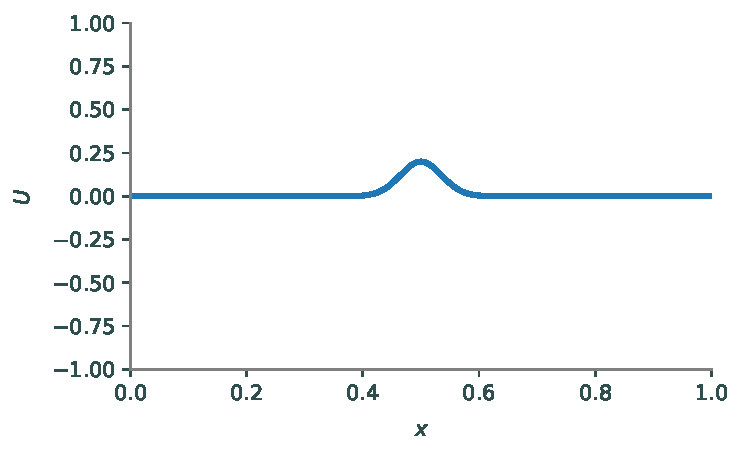
\includegraphics[width=\textwidth]{figures/prob2.pdf}
\caption{$u(x,t=0)$.}
\label{fig:prob2}
\end{figure}
\end{problem}

\begin{problem}
\label{prob:prob3}
Consider the initial boundary value problem
\begin{align*}
	u_{tt} &= u_{xx}, \\
	u(0,t) &= u(1,t) = 0, \\
	u(x,0) &= 0.2e^{-m^2 \left(x - \frac 1 2 \right)^2}\\
	u_t(x,0) &= 0.4m^2 \left(x - \frac 1 2\right)e^{-m^2 \left(x - \frac 1 2 \right)^2}.
\end{align*}
The solution of this problem is a Gaussian pulse.
It travels to the right at a constant speed.
This solution models, for example, a wave pulse in a stretched string.
Note that the fixed boundary conditions reflect the pulse back when it meets the boundary.

Numerically approximate the solution $u(x,t)$ for $t \in \left[0, 1\right]$.
Set $m=20$.
Use 200 subintervals in space and 220 in time, and animate your results.
Then use 200 subintervals in space and 180 in time, and animate your results.
Note that the stability condition is not satisfied for the second mesh.
See Figure \ref{fig:waveeqn:prob3}.

\begin{figure}[H]
\centering
\includegraphics[width=\textwidth]{figures/prob3.pdf}
\caption{$u(x,t=0)$.}
\label{fig:waveeqn:prob3}
\end{figure}
\end{problem}

\begin{problem}
Consider the initial boundary value problem
\begin{align*}
	u_{tt} &= u_{xx}, \\
	u(0,t) &= u(1,t) = 0, \\
	u(x,0) &= 0.2e^{-m^2(x-1/2)^2}\\
	u_t(x,0) &= 0.
\end{align*}
The initial condition separates into two smaller, slower-moving pulses, one traveling to the right and the other to the left.
This solution models, for example, a plucked guitar string

Numerically approximate the solution $u(x,t)$ for $t \in \left[0,2\right]$.
Set $m=20$.
Use 200 subintervals in space and 440 in time, and animate your results.
It is rather easy to see that the solution to this problem is the sum of two traveling waves, one traveling to the left and the other to the right, as described earlier.
\end{problem}

\begin{problem}
\label{prob:prob5}
Consider the initial boundary value problem
\begin{align*}
	u_{tt} &= u_{xx}, \\
	u(0,t) &= u(1,t) = 0, \\
	u(x,0) &= \begin{cases} 1/3 & \text{if } 5/11 < x < 6/11,\\
	0 & \text{otherwise}
	\end{cases}\\
	u_t(x,0) &= 0.
\end{align*}

Numerically approximate the solution $u(x,t)$ for $t \in \left[0, 2\right]$.
Use 200 subintervals in space and 440 in time, and animate your results.
Even though the method is second-order and stable for this discretization, since the initial condition is discontinuous there are large dispersive errors.
See Figure \ref{fig:prob5}.

\begin{figure}[H]
\centering
\begin{subfigure}{.49\textwidth}
\centering
\includegraphics[width=\linewidth]{figures/prob5.pdf}
\caption{$u(x,t=0)$.}
\end{subfigure}
%
\begin{subfigure}{.49\textwidth}
\centering
\includegraphics[width=\linewidth]{figures/prob5_t1.pdf}
\caption{$u(x,t = 0.1)$.}
\end{subfigure}
\caption{The graphs for Problem \ref{prob:prob5} at various times $t$.}
\label{fig:prob5}
\end{figure}
\end{problem}

\section*{Traveling Wave Solutions of an Evolution Equation}
Recall that the advection (transport) equation with initial conditions, given by
\begin{align*}
	&{ }u_t + su_x  = 0, \quad -\infty < x < \infty, \\
	&{ }u(x,0) = f(x),
\end{align*}
has as its general solution $u(x,t) = f(x -st)$.
Consider a general evolutionary PDE of the form
\begin{align}
u_t = G(u,u_x, u_{xx}, \ldots).
\label{evol_pde}
\end{align}
An interesting question to ask is whether \eqref{evol_pde} has traveling wave solutions: is there a signal or wave profile $f(x)$, so that $u(x,t) = f(x-st)$ is a solution of \eqref{evol_pde} that carries the signal at a constant speed $s$?
These traveling waves are often significant physically.
For example, in a PDE modeling insect population dynamics a traveling wave could represent a swarm of locusts; in a PDE describing a combustion process a traveling wave could represent an explosion or detonation.

\subsection*{Burgers' equation}
We will examine the process of studying traveling wave solutions using Burgers' equation, a nonlinear PDE from gas dynamics.
It is given by
\begin{align}
	u_t + \left( \frac{u^2}{2} \right)_x = \nu u_{xx},
    \label{eqn:Burgers_pde}
\end{align}
where $u$ and $\nu$ represent the velocity and viscosity of the gas, respectively.
It models both the process of transport with the nonlinear advection term $(u^2/2)_x = u u_x$, as well as diffusion due to the viscosity of the gas ($\nu u_{xx}$).

Let us look for a traveling wave solution $u(x,t) = \hat{u}(x-st)$ for Burgers' equation.
We transform \eqref{eqn:Burgers_pde} into the moving frame $(x,t) \to (\bar{x},\bar{t}) = (x-st, t)$.
In this frame \eqref{eqn:Burgers_pde} becomes
\begin{align*}
	u_{\bar{t}} - s u_{\bar{x}}+ \left(\frac{u^2}{2} \right)_{\bar{x}} = \nu u_{\bar{x}\bar{x}}
\end{align*}

This new frame of reference corresponds to an observer moving along with the wave, so that the wave appears stationary as the observer studies it.
Thus, $\hat{u}_{\bar{t}} = 0$, so that the wave profile $\hat{u}$ satisfies the ordinary differential equation
\begin{align}
	 -s u_{\bar{x}}+ \left(\frac{u^2}{2} \right)_{\bar{x}} = \nu u_{\bar{x}\bar{x}}.
	\label{eqn:Burgers_ode}
\end{align}

From here on we will drop the bar notation for simplicity.
We seek a traveling wave solution with asymptotically constant boundary conditions; that is,  $\lim_{x \to \pm \infty}\hat{u}(x) = u_{\pm}$ both exist, and  $\lim_{x \to \pm \infty} \hat{u}'(x) = 0$.
We will suppose that $u_- > u_+ > 0$.

Note that to this point we still don't know the speed of the traveling wave.
Integrating both sides of this differential equation, and then taking the limit as $x \to +\infty$, we obtain
\begin{align*}
-s\int_{-\infty}^x u' + \int_{-\infty}^x \left(\frac{u^2}{2}\right)' &= \nu \int_{-\infty}^x u'',\\
-s(u(x) - u_-) + \frac{u^2(x)}{2} - \frac{u_-^2}{2} &= \nu (u'(x) - u'(-\infty)), \\
-s(u_+ - u_-) + \frac{u_+^2}{2} - \frac{u_-^2}{2} &= 0.
\end{align*}
Thus given boundary conditions $u_{\pm}$ at $\pm \infty$, the speed of the traveling wave must be $s = \frac{u_- + u_+}{2}$.

Usually at this point, the traveling wave must be numerically solved using the profile ODE (\eqref{eqn:Burgers_ode} for Burgers equation).
However, the profile ODE for Burgers' is simple enough that it is possible to obtain an analytic solution.
The traveling wave is  given by
\begin{align}
\hat{u}(x) = s - a \tanh \left(\frac{ax }{2\nu} + \delta\right)
\label{eqn:waveeqn:uhat}
\end{align}
where $a = (u_- - u_+)/2$ and $\delta$ is a fixed real number.
We get a family of solutions because any translation of a traveling wave solution is also a traveling wave solution.

\subsection*{Stability of traveling waves}
Suppose that an evolutionary PDE
\begin{align}
u_t = G(u,u_x, u_{xx}, \ldots).
\label{eqn:evol_pde_repeat}
\end{align}
has a traveling wave solution $u(x,t) = \hat{u}(x-st)$.
An interesting question to consider is whether the mathematical solution, $\hat{u}$, has a physical analogue.
In other words, does the traveling wave show up in real life?
This question is the start of the mathematical study of stability of traveling waves.

We begin by translating \eqref{eqn:evol_pde_repeat} into the moving frame $(x,t) \to (\bar{x},\bar{t}) = (x-st, t)$.
In this frame the PDE becomes
\begin{align*}
u_t - su_x = G(u,u_x, u_{xx}, \ldots).
\end{align*}
In these coordinates the traveling wave is stationary.
Thus, the solution of
\begin{align*}
\begin{split}
u_t - su_x &= G(u,u_x, u_{xx}, \ldots), \\
u(x,t = 0) &= \hat{u}(x),
\end{split}
\end{align*}
is given by $u(x,t) = \hat{u}(x)$.
We say that the traveling wave $\hat{u}$ is asymptotically orbitally stable if whenever $v(x)$ is a small perturbation of $\hat{u}(x)$, the general solution of
\begin{align*}
\begin{split}
u_t - su_x &= G(u,u_x, u_{xx}, \ldots), \\
u(x,t = 0) &= v(x),
\end{split}
\end{align*}
converges to some translation of $\hat{u}$ as $t \to \infty$.
Using this definition to prove stability of a traveling wave is a nontrivial task.

\subsection*{Visualizing stability of the traveling wave solution of Burgers' equation}
The traveling wave solution of Burgers' equation is a stable wave.
To view this numerically, we discretize the PDE
\[u_t -su_x + uu_x = u_{xx}\]
using the second-order centered approximations
\begin{align*}
&{ } D_t U_j^{m+1/2} = \frac{U_j^{m+1}-U_j^m}{\Delta t}, \quad
D_{xx}U_j^{m+1/2} = \frac{1}{2} \left( \frac{U_{j+1}^{m+1}-U_{j-1}^{m+1}}{2 \Delta x} +  \frac{U_{j+1}^{m}-U_{j-1}^{m}}{2 \Delta x}\right),\\
&{ } D_{xx}U_j^{m+1/2} = \frac{1}{2} \left( \frac{U_{j+1}^{m+1}- U_{j}^{m+1}+U_{j-1}^{m+1}}{(\Delta x)^2} + \frac{U_{j+1}^{m}- U_{j}^{m}+U_{j-1}^{m}}{(\Delta x)^2}\right).
\end{align*}

Substituting these expressions into the PDE we obtain a second-order, implicit Crank--Nicolson method
\begin{align}
\begin{split}
\label{waveeqn:eqn:crank-nicolson}
U_j^{m+1} - U_j^m &= K_1 \big[(s - U_j^{m+1})(U_{j+1}^{m+1} - U_{j-1}^{m+1})
+ (s - U_j^m) (U_{j+1}^m - U_{j-1}^m) \big] \\
&+ K_2 \big[(U_{j+1}^{m+1} - 2U_j^{m+1}+ U_{j-1}^{m+1}) + (U_{j+1}^m -2U_j^m + U_{j-1}^m) \big]
\end{split}
\end{align}
where $K_1 = \frac{ \Delta t }{4 \Delta x}$ and $K_2 = \frac{ \Delta t}{2(\Delta x)^2}$.

Unlike the previous problems, this equation is implicit in $U^{m+1}$.
That is, we can't solve each iteration for the next step $U^{m+1}$ explicitly.
Instead, we'll need to use a root-finding algorithm like Newton's method.

\begin{problem}
\label{prob:prob6}
Numerically solve the initial value problem
\begin{align*}
	&{ } u_t -su_x + uu_x = u_{xx}, \quad x \in (-\infty,\infty),\\
	&{ } u(x,0) = \hat{u}(x)+v(x),
\end{align*}
for $t \in [0,1]$, where $\hat{u}$ is given in \eqref{eqn:waveeqn:uhat} with $\nu=1$ and $\delta=0$.
Let the perturbation $v(x)$ be given by
\[v(x) = 3.5(\sin{(3x)} + 1)\frac{1}{\sqrt{2\pi}} \exp{(-x^2/2)}.\]
Approximate the $x$ domain, $(-\infty, \infty)$, numerically by the finite interval $[-20,20]$, and fix $u(-20) = u_-$, $u(20) = u_+$.
Let $u_- = 5$, $u_+ = 1$ which makes $s = 3$.
Use 150 intervals in space and 350 steps in time.
Animate your solution $U$.
Also include in your animation the original traveling wave $\hat u$.
You should see the solution converge to a translate of $\hat{u}$.
See Figure \ref{fig:prob6}.
For your root-finding algorithm, use \li{scipy.optimize.fsolve}.

Hint:
To solve for each $U^{m+1}$, define a function \li{cranknicolson} that accepts a guess for $U^{m+1}$ and returns the expression obtained from moving all the terms in \eqref{waveeqn:eqn:crank-nicolson} to one side (call the expression $\tilde U$).
At each iteration, use \li{fsolve} to find the value of $U^{m+1}$ that makes $\tilde U = \0\,$---that is, it solves \eqref{waveeqn:eqn:crank-nicolson}.
You can use $U^m$ as a good guess.

We still need to enforce the boundary conditions.
Before returning $\tilde U$, set the value of, for example, the first value $\tilde U_0$ to be $U^{m+1}_0 - u_-$. This will ensure \li{fsolve} finds $U^{m+1}$ such that $U^{m+1}_0 = u_-$.

Also note that \li{fsolve} accepts an additional parameter \li{args} that it passes to the function whose root it is finding.
You might consider setting up \li{cranknicolson} to accept the previous value $U^m$.

\begin{figure}[H]
\centering
\begin{subfigure}{.49\textwidth}
\centering
\includegraphics[width=\linewidth]{figures/prob6_initial.pdf}
\caption{$u(x,t=0)$.}
\end{subfigure}
%
\begin{subfigure}{.49\textwidth}
\centering
\includegraphics[width=\linewidth]{figures/prob6_ufinal_utilda.pdf}
\caption{$u(x,t = 1)$ vs $\hat{u}$.}
\end{subfigure}
\caption{The graphs for Problem \ref{prob:prob6}.}
\label{fig:prob6}
\end{figure}
\end{problem}

\section*{Two-Dimensional Wave}

Consider the two-dimensional wave equation:
\begin{align}
\label{waveeqn:eqn:2d-wave-eqn}
u_{tt} &= \alpha^2 \nabla^2 u = \alpha^2 (u_{xx} + u_{yy}) \\
\label{waveeqn:eqn:2d-wave-eqn-boundary-conditions}
u(x, y, t) &= 0, \quad (x, y) \in \partial \big([x_0, x_f] \times [y_0, y_f]\big) \\
\begin{split}
	\label{waveeqn:eqn:2d-wave-eqn-initial-conditions}
	u(x, y, 0) &= f(x, y) \\
	u_t(x, y, 0) &= g(x, y)
\end{split}
\end{align}
for some real, non-negative $\alpha$.

As with the one-dimensional wave equation, we'll use the second-order centered difference approximations (as in \eqref{waveeqn:eqn:2nd-order-centered-2nd-derivative}) for each of the second derivatives.
Let $U_{i,j}^m$ be the numerical approximation for $u(x_i, y_j, t_m)$.
% TODO: It'd be nice to add Big O around here.
We can approximate \eqref{waveeqn:eqn:2d-wave-eqn} with
\begin{equation*}
	\frac {U_{i,j}^{m+1} - 2 U_{i,j}^m + U_{i,j}^{m-1}} {(\Delta t)^2}
	= \alpha^2 \left[
		\frac {U_{i+1,j}^m - 2 U_{i,j}^m + U_{i-1,j}^m} {(\Delta x)^2}
		+ \frac {U_{i,j+1}^m - 2 U_{i,j}^m + U_{i,j-1}^m} {(\Delta y)^2}
	\right].
\end{equation*}
Assuming the same step size in each spatial dimension $h = \Delta x = \Delta y$, we can rearrange:
\begin{align}
	\nonumber
	U_{i,j}^{m+1} &= \frac {\alpha^2 (\Delta t)^2} {h^2} (
		U_{i+1,j}^m - 2 U_{i,j}^m + U_{i-1,j}^m + U_{i,j+1}^m - 2 U_{i,j}^m + U_{i,j-1}^m
	) + 2 U_{i,j}^m - U_{i,j}^{m-1}\\
	\label{waveeqn:eqn:2d-wave-eqn-vectorized}
	&= \lambda \left(
		U_{i+1,j}^m + U_{i-1,j}^m + U_{i,j+1}^m + U_{i,j-1}^m - 4 U_{i,j}^m
	\right) + 2 U_{i,j}^m - U_{i,j}^{m-1}
\end{align}
where $\lambda = \frac {\alpha^2 (\Delta t)^2} {h^2}$.
Assume there are $N$ subintervals in each spatial dimension so that there are $N+1$ points, $x_0 < \ldots < x_N$ and $y_0 < \ldots < y_N$.
Because of our homogeneous Dirichlet boundary conditions \eqref{waveeqn:eqn:2d-wave-eqn-boundary-conditions}, we have $U_{i, j}^m = 0$ for $i = 0, N$ or $j = 0, N$, so we can just compute $U_{i, j}^{m+1}$ for $1 \le i \le N-1$ and $1 \le j \le N-1$, and ignore $U_{i, j}^m$ terms on the boundary.
We'll flatten each $U^m$ and write this scheme as the matrix equation
\begin{equation}
	\label{waveeqn:eqn:2d-wave-eqn-matrix}
    U^{m+1} = A U^{m} - U^{m-1}
\end{equation}
where
\begin{align*}
A &=
\begin{bmatrix}
	T 		& \Lambda &  		& \\
	\Lambda & T 	  & \Lambda & \\
			& \ddots  & \ddots  & \Lambda \\
			&		  & \Lambda & T
\end{bmatrix} \\
\Lambda &= \lambda I \\
T &=
\begin{bmatrix}
	2 - 4 \lambda & \lambda 	  &			& 		 		& \\
	\lambda 	  & 2 - 4 \lambda & \lambda & 				& \\
				  & \ddots 		  & \ddots 	& \ddots 		& \\
				  &				  & \lambda & 2 - 4 \lambda & \lambda \\
				  &				  & 		& \lambda		& 2 - 4 \lambda
\end{bmatrix}.
\end{align*}
We have that $T$ and $\Lambda$ are both $(N-1) \times (N-1)$, and each $U^m$ has length $(N-1)^2$.
Note that we may flatten each $U^m$ either by columns or by rows due to the spatial symmetry of \eqref{waveeqn:eqn:2d-wave-eqn-vectorized}.

However, for a given time step our iterative matrix algorithm \eqref{waveeqn:eqn:2d-wave-eqn-matrix} requires two previous time steps, so for the first time step we'll need a different method.
We'll start with a Taylor approximation centered at $t = 0$ and then use \eqref{waveeqn:eqn:2d-wave-eqn} and \eqref{waveeqn:eqn:2d-wave-eqn-initial-conditions}:
\begin{align*}
	u(x, y, \Delta t) &= u(x, y, 0) + \Delta t \, u_t(x, y, 0) + \frac{(\Delta t)^2} 2 u_{tt}(x, y, 0) + \mathcal O\left((\Delta t)^3\right) \\
	&= u(x, y, 0)
		+ \Delta t \, g(x, y)
		+ \frac{(\Delta t)^2}2 \alpha^2 \nabla^2 u(x, y, 0)
		+ \mathcal O\left((\Delta t)^3\right).
\end{align*}
We then expand the last term using second-order centered second-derivative approximations as in \eqref{waveeqn:eqn:2nd-order-centered-2nd-derivative}:
\begin{align*}
	\frac{(\Delta t)^2}2 \alpha^2 \nabla^2 u(x, y, 0)
	&= \frac{\alpha^2 (\Delta t)^2}2 \big(
		u_{xx}(x, y, 0) + u_{yy}(x, y, 0)
		\big) \\
	&= \frac{\alpha^2 (\Delta t)^2}2 \bigg(
			\frac{u(x + h, y, 0) - 2 u(x, y, 0) + u(x - h, y, 0)}{h^2} \\
			& \hphantom{{}={} \frac{\alpha^2 (\Delta t)^2}2 \bigg(}
			\mathllap{{}+{}} \frac{u(x, y + h, 0) - 2 u(x, y, 0) + u(x, y - h, 0)}{h^2}
			+ \mathcal O\left((\Delta t)^2\right) \bigg) \\
	&= \frac{\alpha^2 (\Delta t)^2}{2 h^2} \bigg(
			u(x + h, y, 0) + u(x - h, y, 0) \\
			& \hphantom{{}={} \frac{\alpha^2 (\Delta t)^2}{2 h^2} \bigg(}
			\mathllap{{}+{}} u(x, y + h, 0) + u(x, y - h, 0)
			- 4 u(x, y, 0)
		\bigg) + \mathcal O\left((\Delta t)^4\right).
\end{align*}
Using our $U_{i, j}^m$ notation, $u(x, y, \Delta t)$ becomes
\begin{equation*}
	U_{i, j}^1 = U_{i, j}^0 + \Delta t \, g(x, y)
		+ \frac{\lambda}{2} \left(
			U_{i+1, j}^0 + U_{i-1, j}^0 + U_{i, j+1}^0 + U_{i, j-1}^0 - 4 U_{i, j}^0
	\right) + \mathcal O\left((\Delta t)^3\right).
\end{equation*}

\begin{problem}
\label{waveeqn:prob:2d-wave-eqn}
Solve the 2D wave equation \eqref{waveeqn:eqn:2d-wave-eqn}.
Use $N = 200$ spatial subintervals and $M = 500$ time subintervals.
Use a spatial domain $(x, y) \in [-10, 10] \times [-10, 10]$ and a time domain $t \in (t_0, t_f) = (0, 40)$.
Set $f(x, y) = 3 \frac 1 {2 \pi} \exp \left(-\frac12 \left(x^2 + y^2
\right) \right)$, and set $g(x, y) = 0$.
Finally, use $\alpha = 0.8$.
Animate the result, and compare with Figure \ref{waveeqn:fig:prob7}.
Remember to use sparse matrices.

Hint: You may find useful the functions \li{scipy.sparse.diags}, \mbox{\li{scipy.sparse.block_diag},} and \li{<sparse_matrix>.setdiag}.
Also note that $f(x, y)$ is equal to 3 times the probability density function of the standard two-dimensional normal distribution.
\end{problem}

\begin{figure}[H]
	\centering
	\includegraphics[width=\textwidth]{figures/prob7.pdf}
	\caption{The solution to Problem 7 (the 2D wave equation) $u(x, y, t=6)$.}
	\label{waveeqn:fig:prob7}
\end{figure}